\section{Evaluation of Preprocessing Pipelines and Heuristics}

%\section{Which Preprocessing Approach To Prefer}
\label{sec:which_preprocessing}

\todo{ARRIVED HERE -- need to merge section 4 and 7.}

We further investigate the preprocessing steps with the groups of features introduced in Table~\ref{tab:doc_features}.
For that, we present in Figure~\ref{fig:boxplot_corr_docs} the box plot of Spearman rank correlation metric divided by preprocessing alternative for CLEF eHealth 2015 and 2016\footnote{Due to space limitation, additional plots with Pearson and Kendall correlations are available online at \url{XYZ}.}.
%Figures~\ref{fig:boxplot_corr_docs_2015} and~\ref{fig:boxplot_corr_docs_2016} the box plot of different correlation metrics divided by preprocessing alternative for CLEF eHealth 2015 and 2016. 
For instance, the very first box plot in the upper part of these figures shows the absolute Pearson's rank correlation of different readability metrics when using a combination of Naive and ForcePeriod as preprocessing steps.
Boxes extend from the lower to upper quartile values of the data, with a line at the median. Whiskers extend from the box to show the range of the data. Flier points are those past the end of the whiskers, usually interpreted as outlier values.




%We also include in Figures~\ref{fig:boxplot_corr_docs_2015} and~\ref{fig:boxplot_corr_docs_2016} 
We also include in Figure~\ref{fig:boxplot_corr_docs} 
boxes for the summary of the 3 preprocessing procedures to remove HTML, the use of HTML features, which is done without any preprocessing and the comparison with other human assessors. For CLEF eHealth 2015, we used as human assessments the additional assessments made by unpaid medical students and health consumers (see~\cite{palotti16b}), while for CLEF eHealth 2016 data, we randomly selected 100 pages that were assessed by another assessor. \mytodo{add at least another person doing assessments}.
The correlations with human assessments provide important insights on how hard and subjective understandability assessments are.

\begin{figure*}[h!]
   \centering
   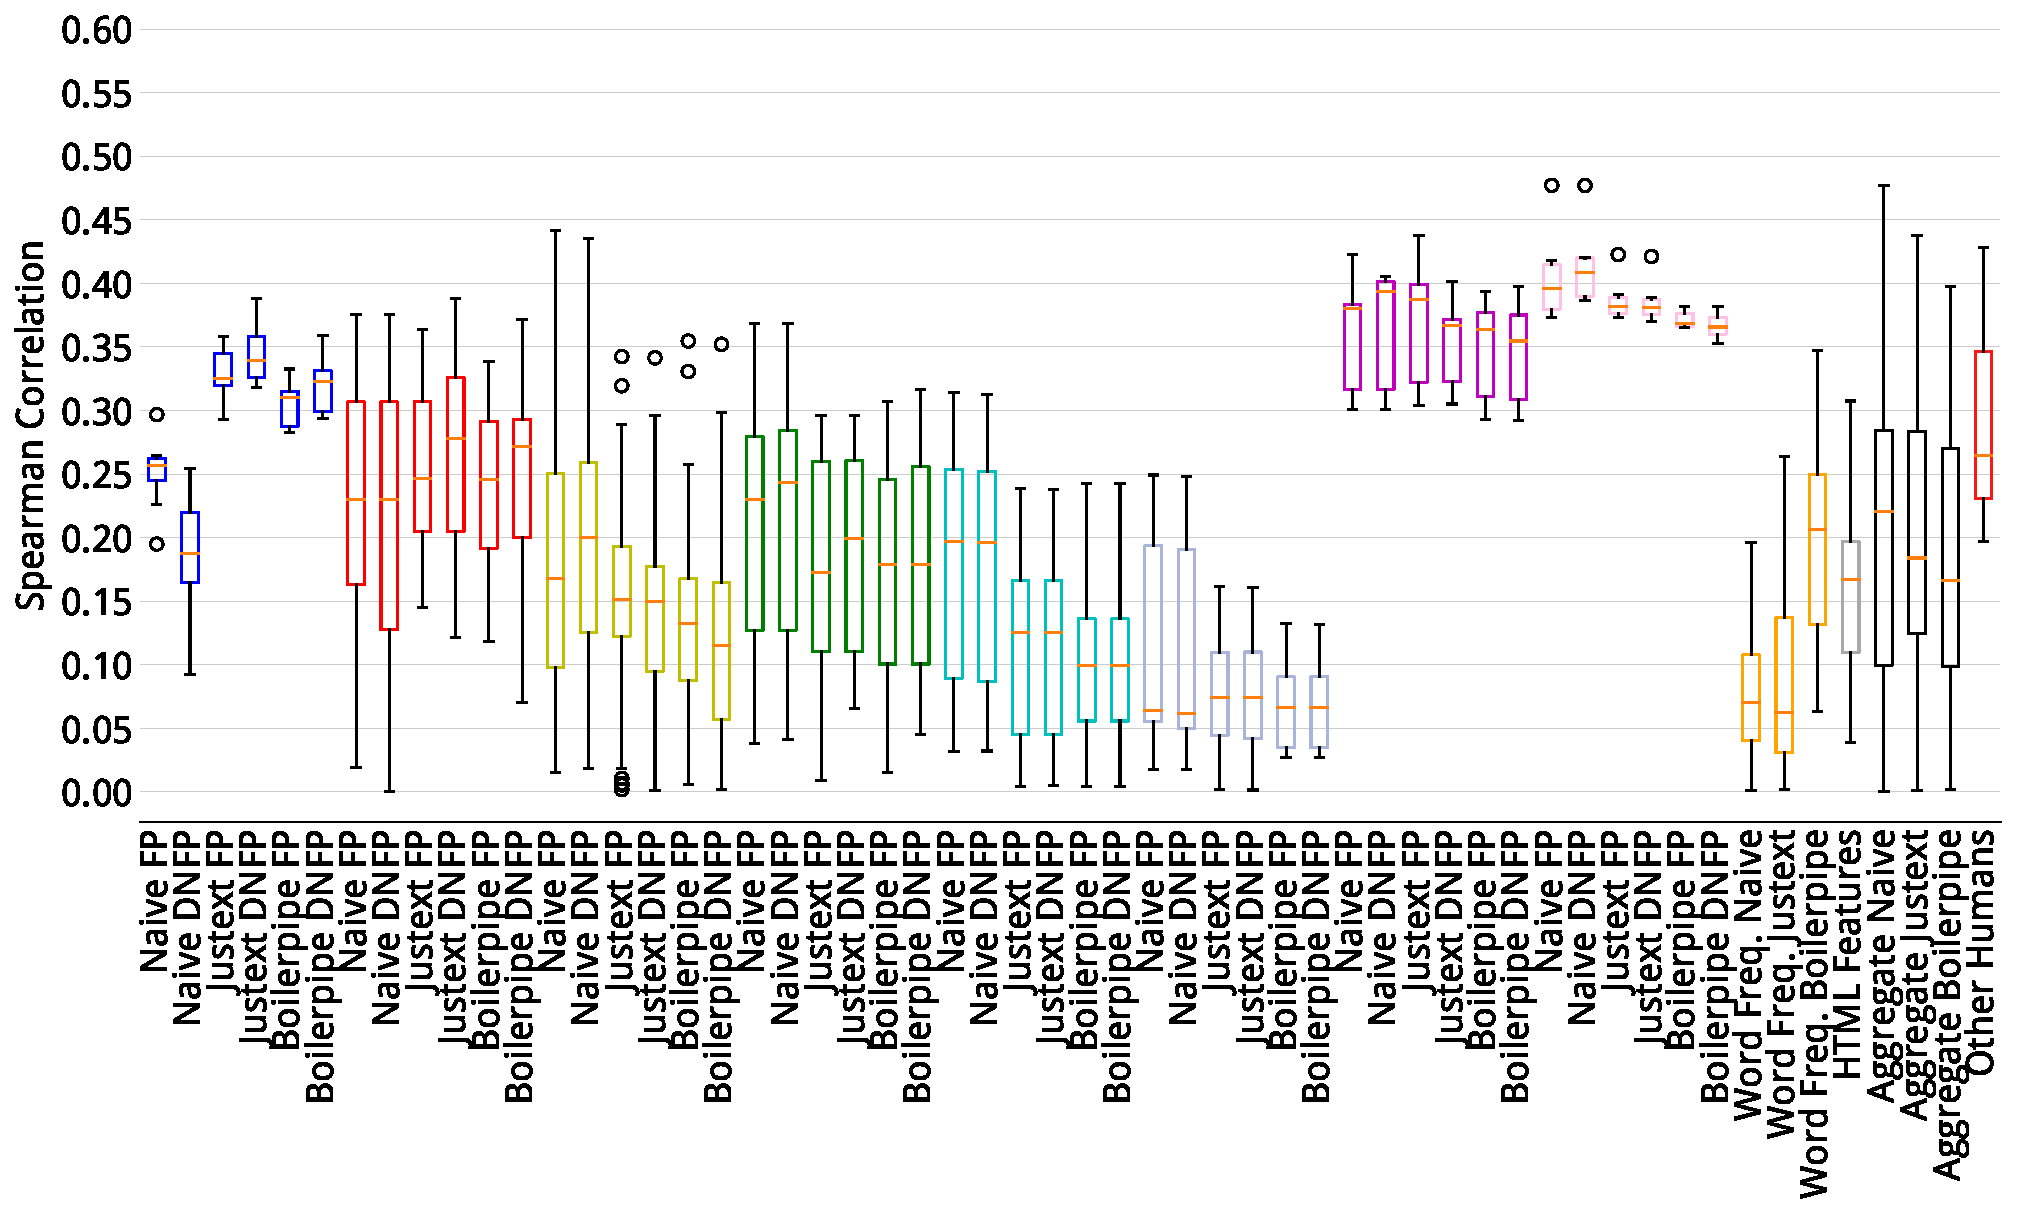
\includegraphics[width=0.80\textwidth]{graphics/box_spearman15_raw_values}
   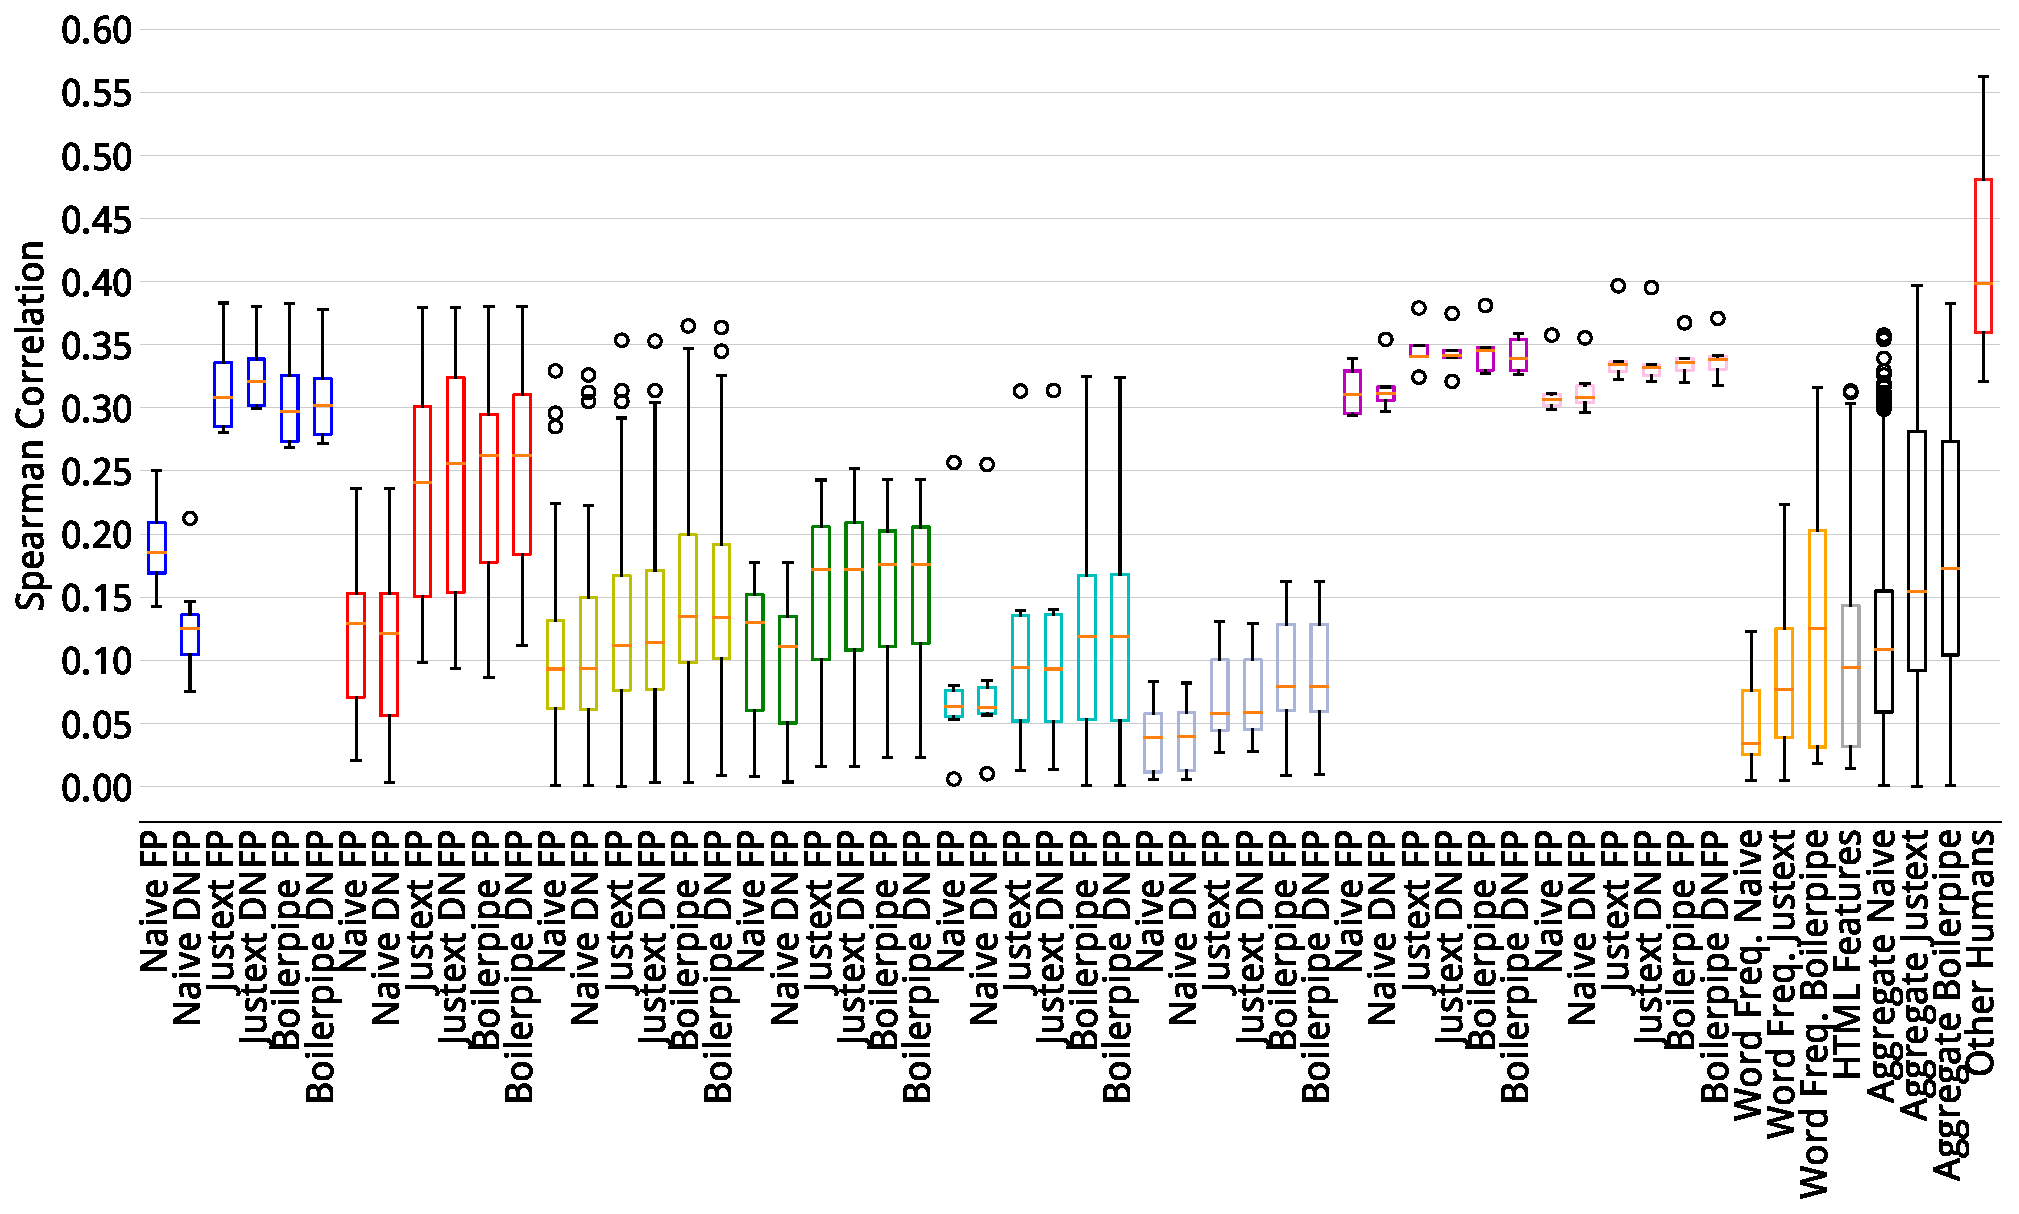
\includegraphics[width=0.80\textwidth]{graphics/box_spearman16_raw_values}
   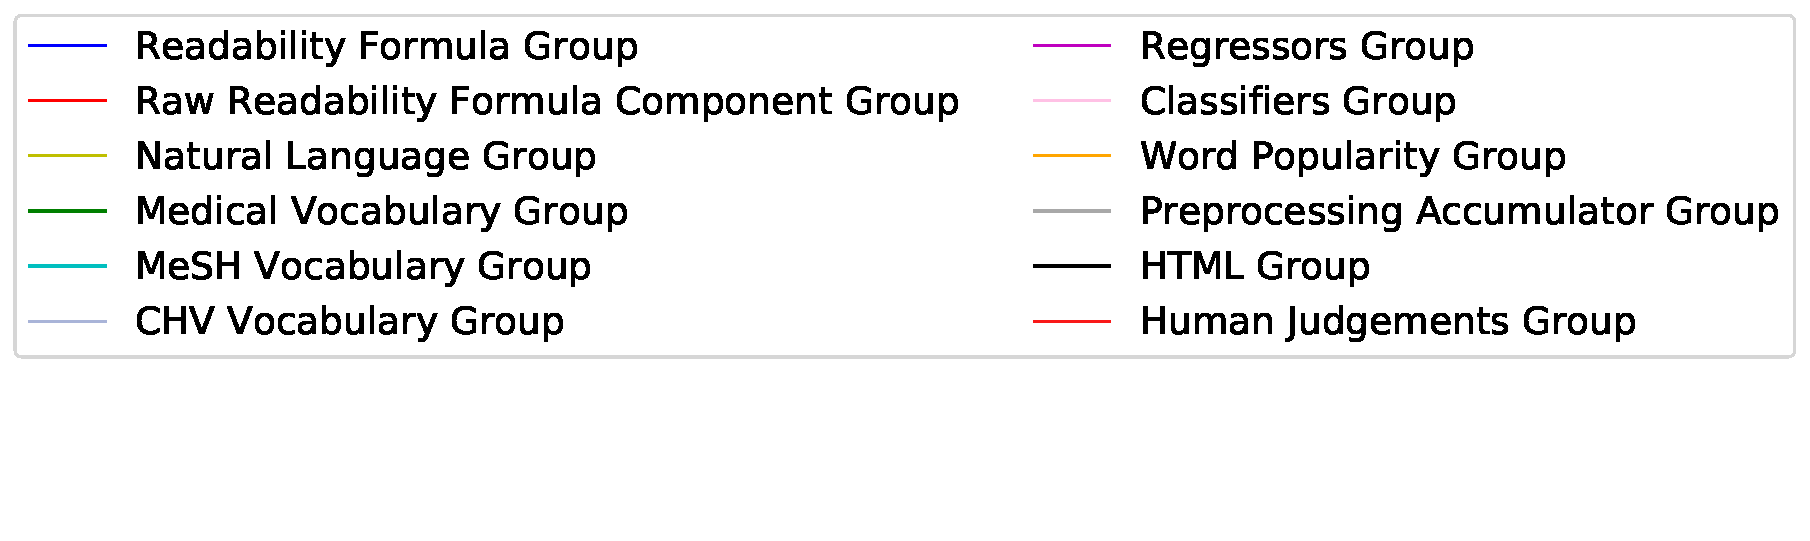
\includegraphics[width=0.7\textwidth]{graphics/legendCorr}
   \vspace{-1cm}
   \caption{Box plots divided by feature groups. Correlations are calculated using understandability labels from relevant documents assessed in CLEF eHealth 2015 (top) and 2016 (bottom).}
   \label{fig:boxplot_corr_docs}
\end{figure*}

%
%\begin{figure*}[th!]
%   \centering
%   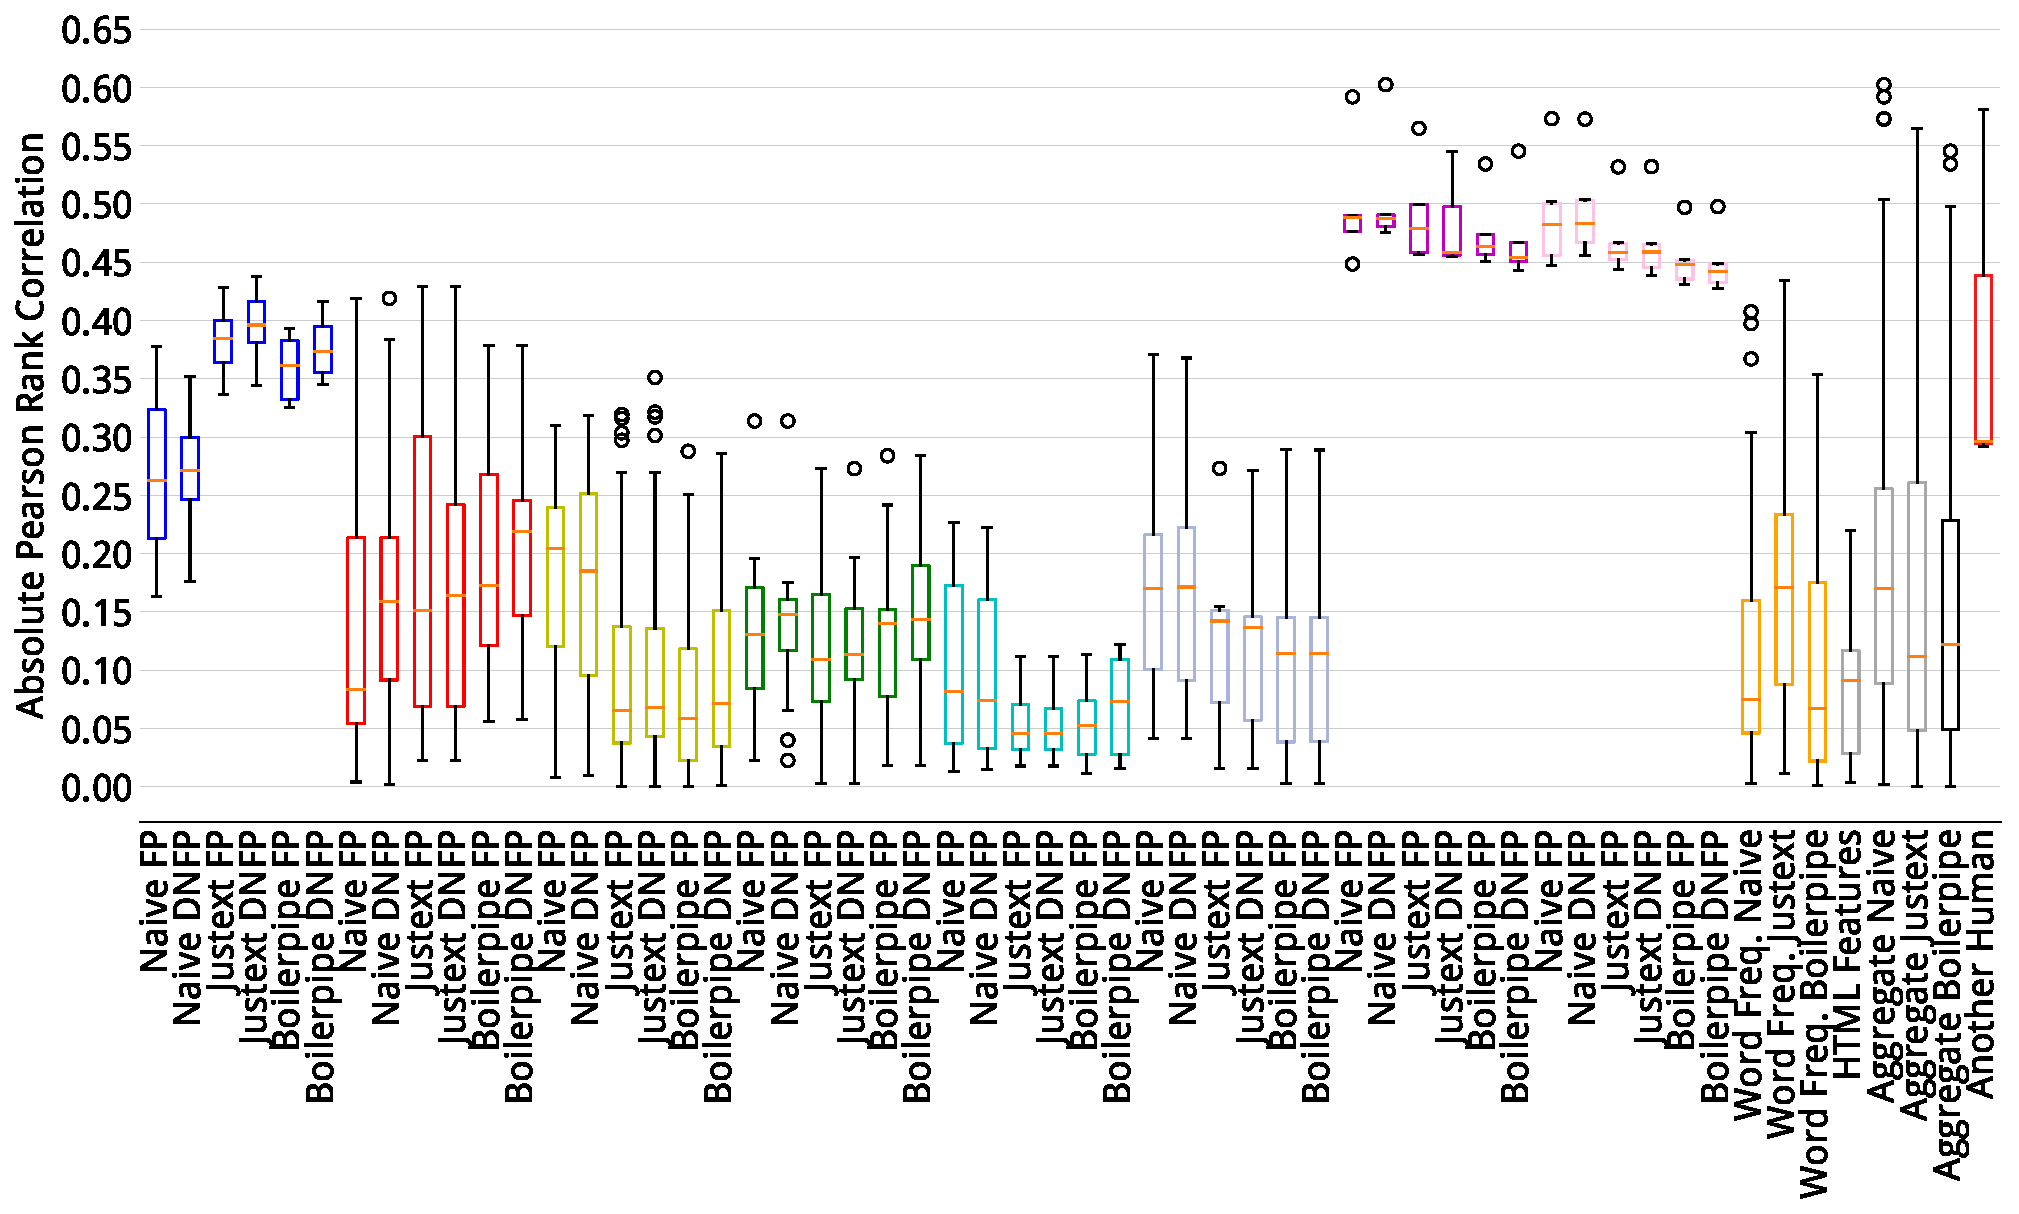
\includegraphics[width=0.90\textwidth]{graphics/box_pearson15_raw_values}
%   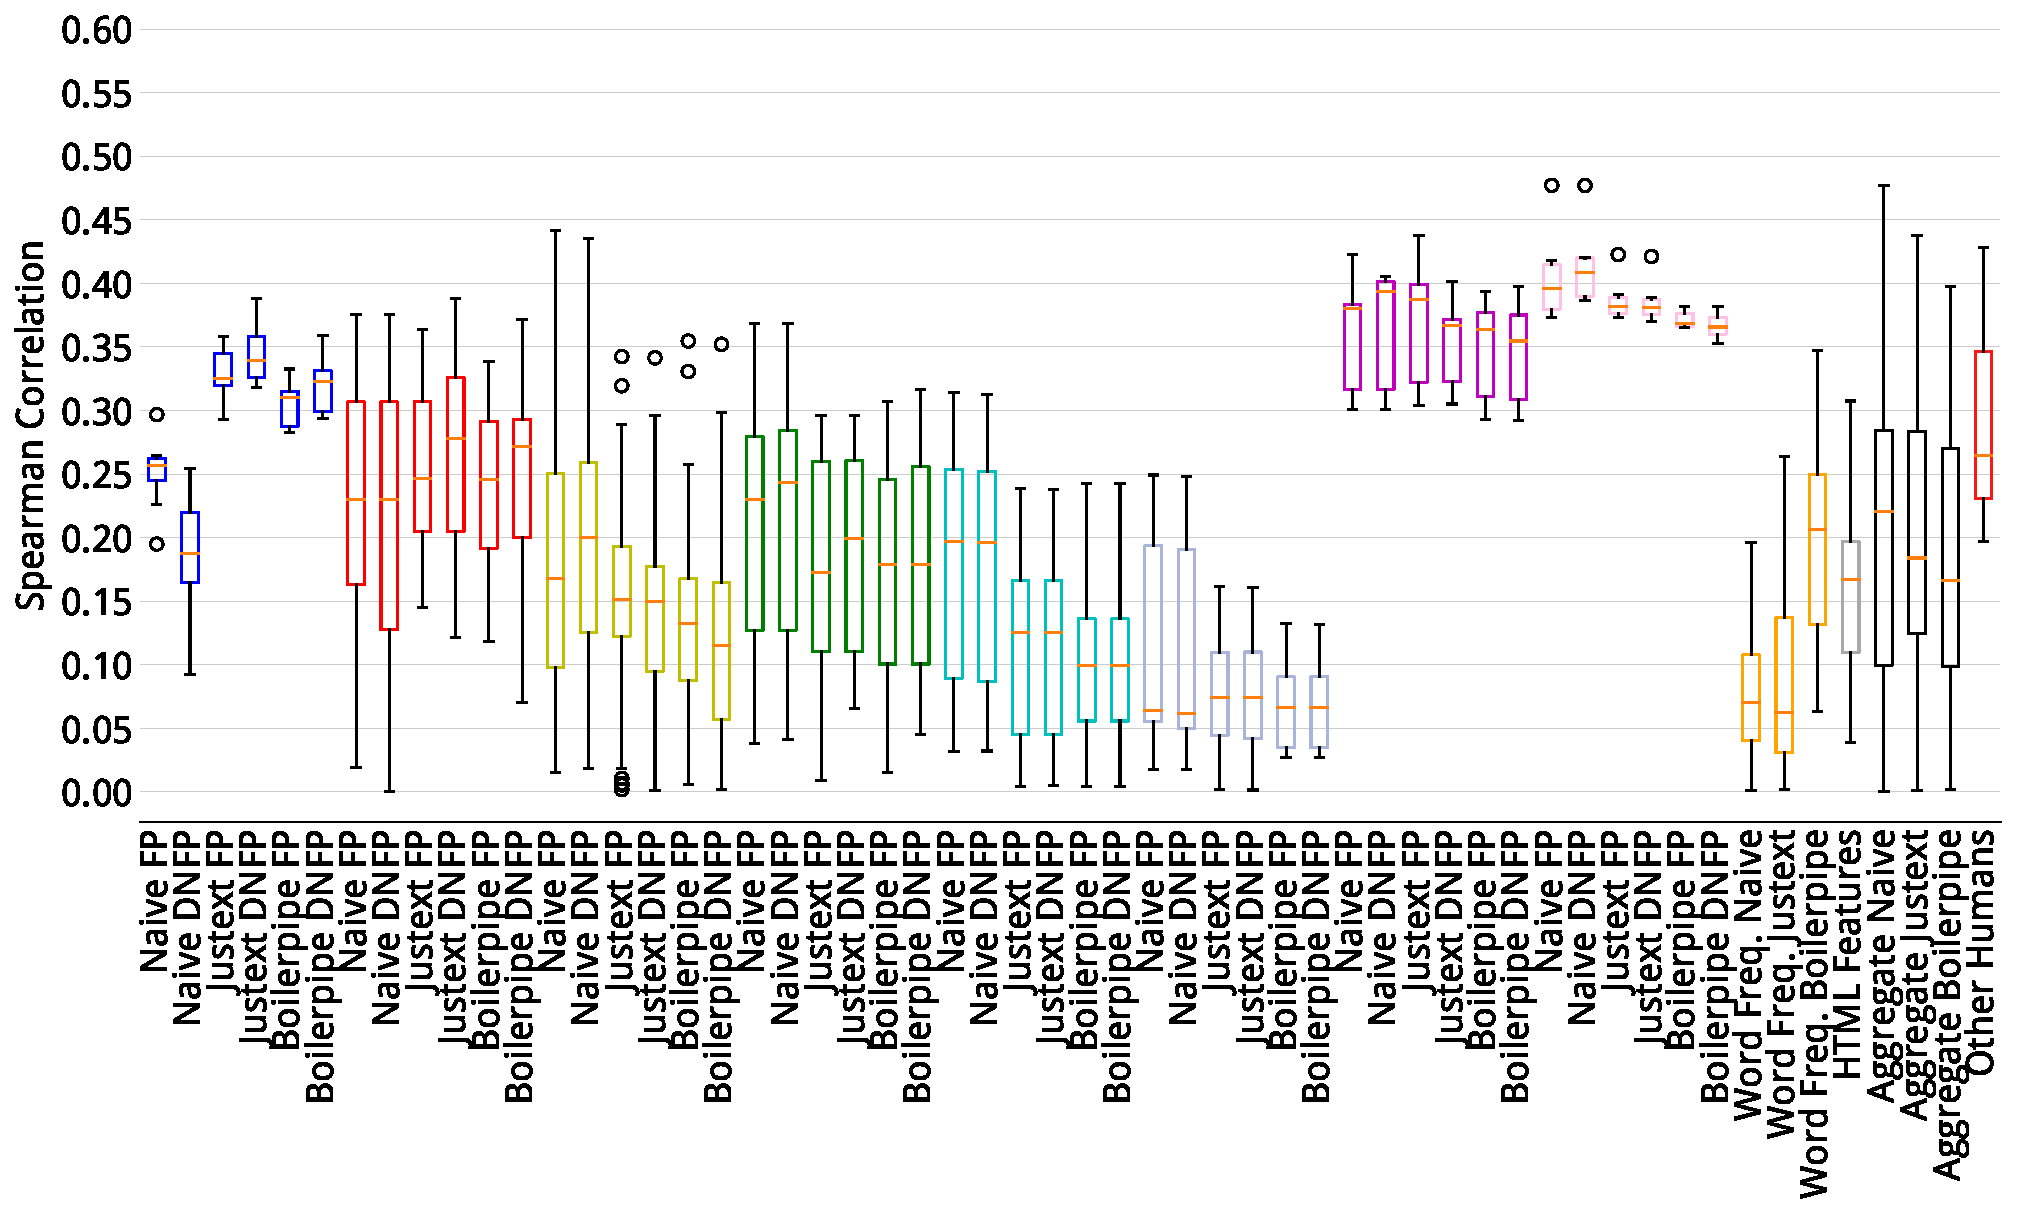
\includegraphics[width=0.90\textwidth]{graphics/box_spearman15_raw_values}
%   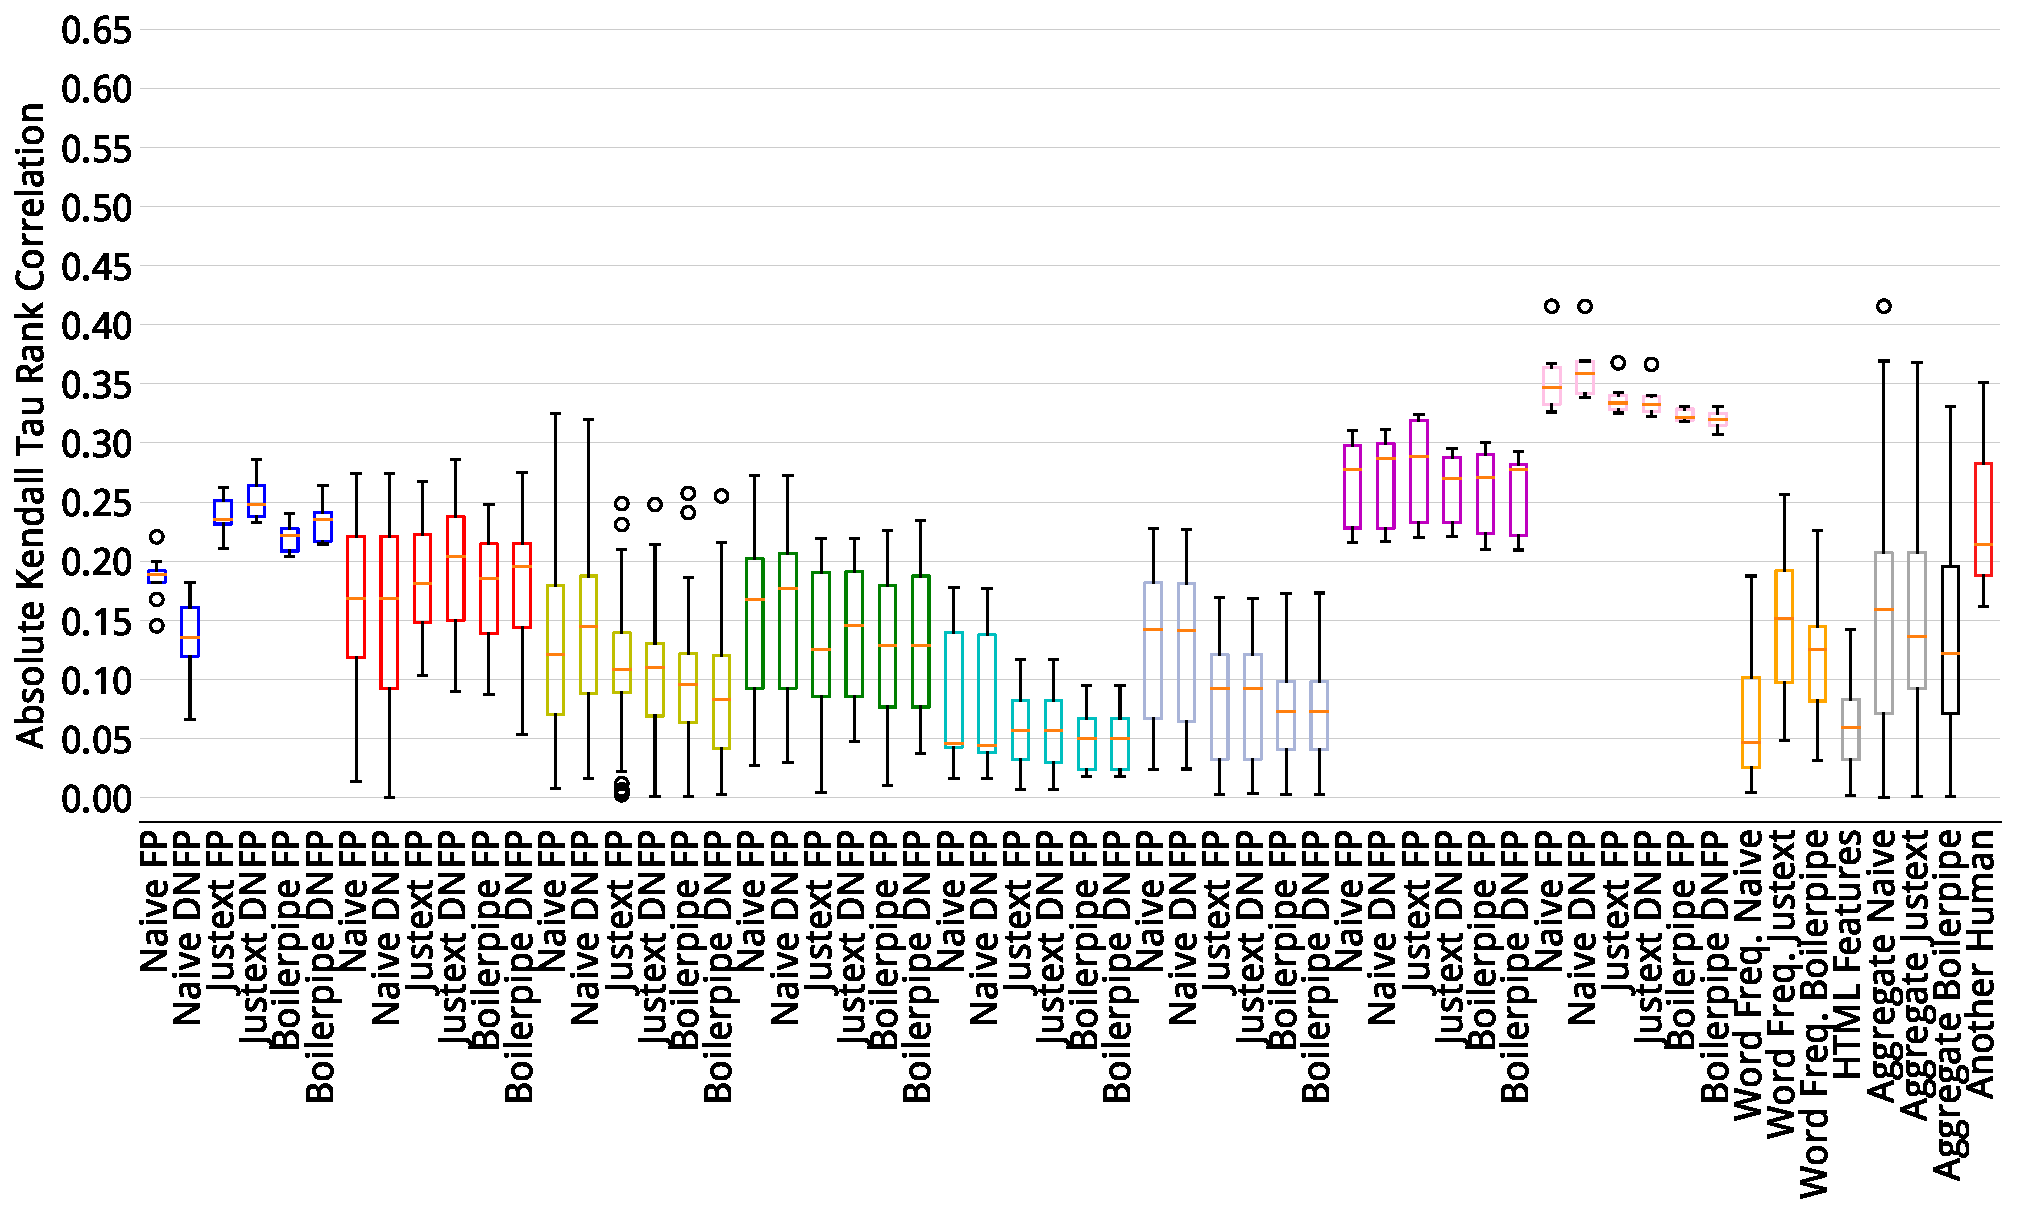
\includegraphics[width=0.90\textwidth]{graphics/box_kendalltau15_raw_values}
%   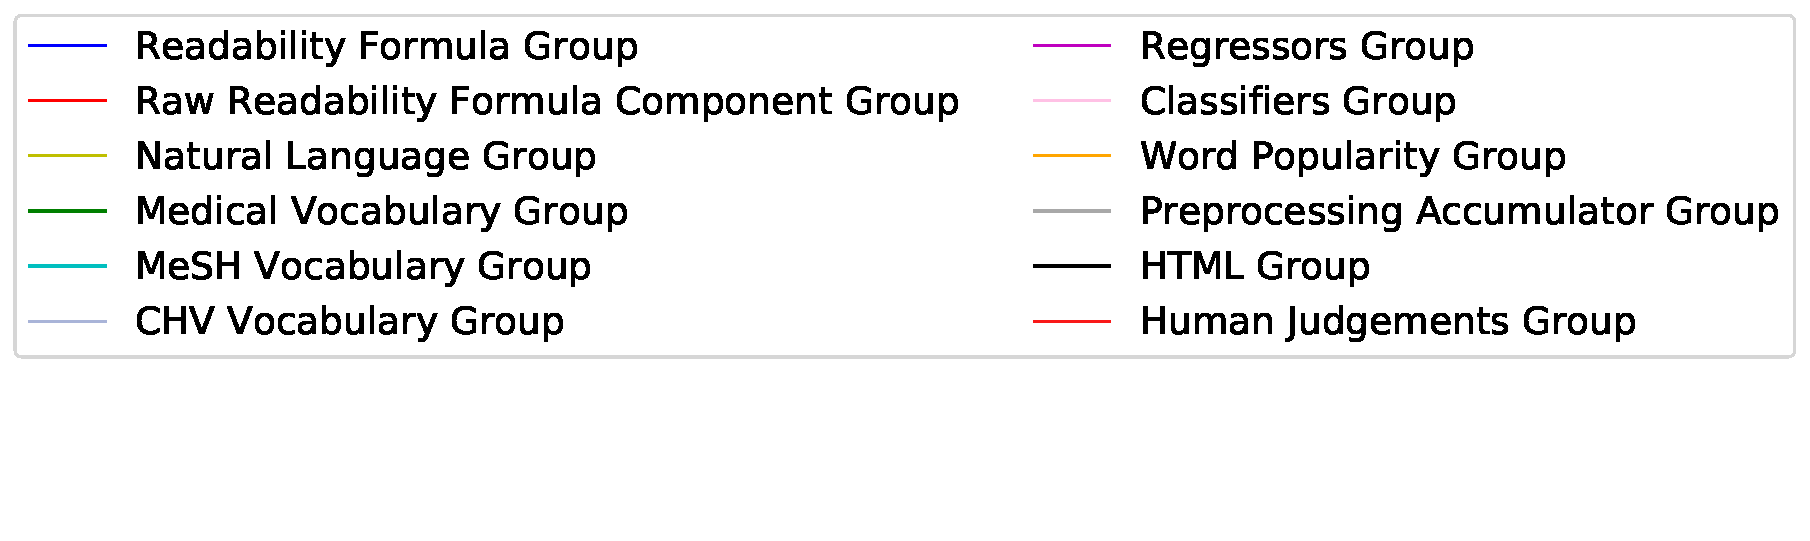
\includegraphics[width=0.65\textwidth]{graphics/legendCorr}
%   \caption{Box plots divided by feature groups. Correlations are calculated using understandability labels from relevant documents assessed in CLEF eHealth 2015}
%   \label{fig:boxplot_corr_docs_2015}
%\end{figure*}

%\begin{figure*}[th!]
%   \centering
%   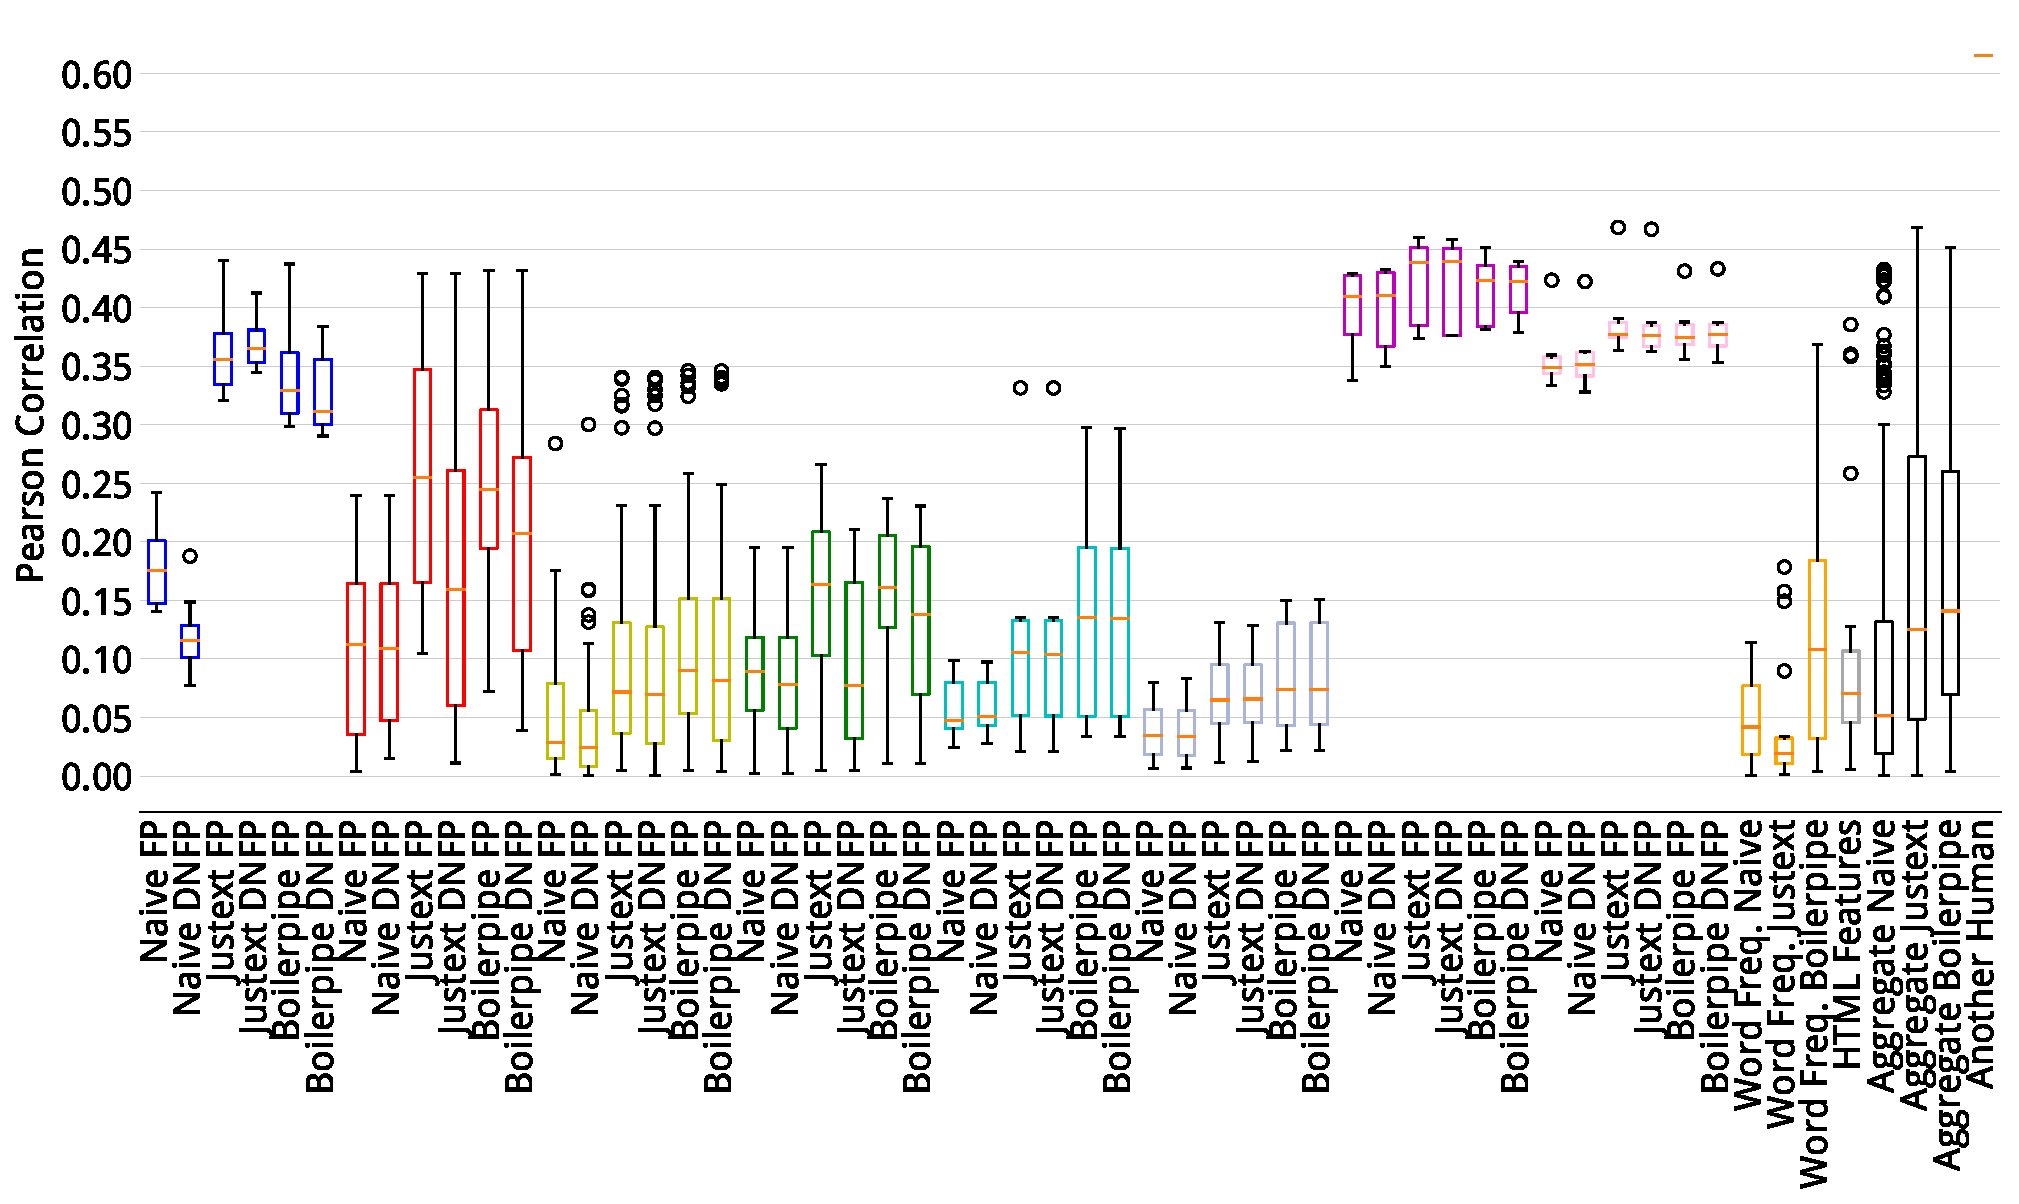
\includegraphics[width=0.90\textwidth]{graphics/box_pearson16_raw_values}
%   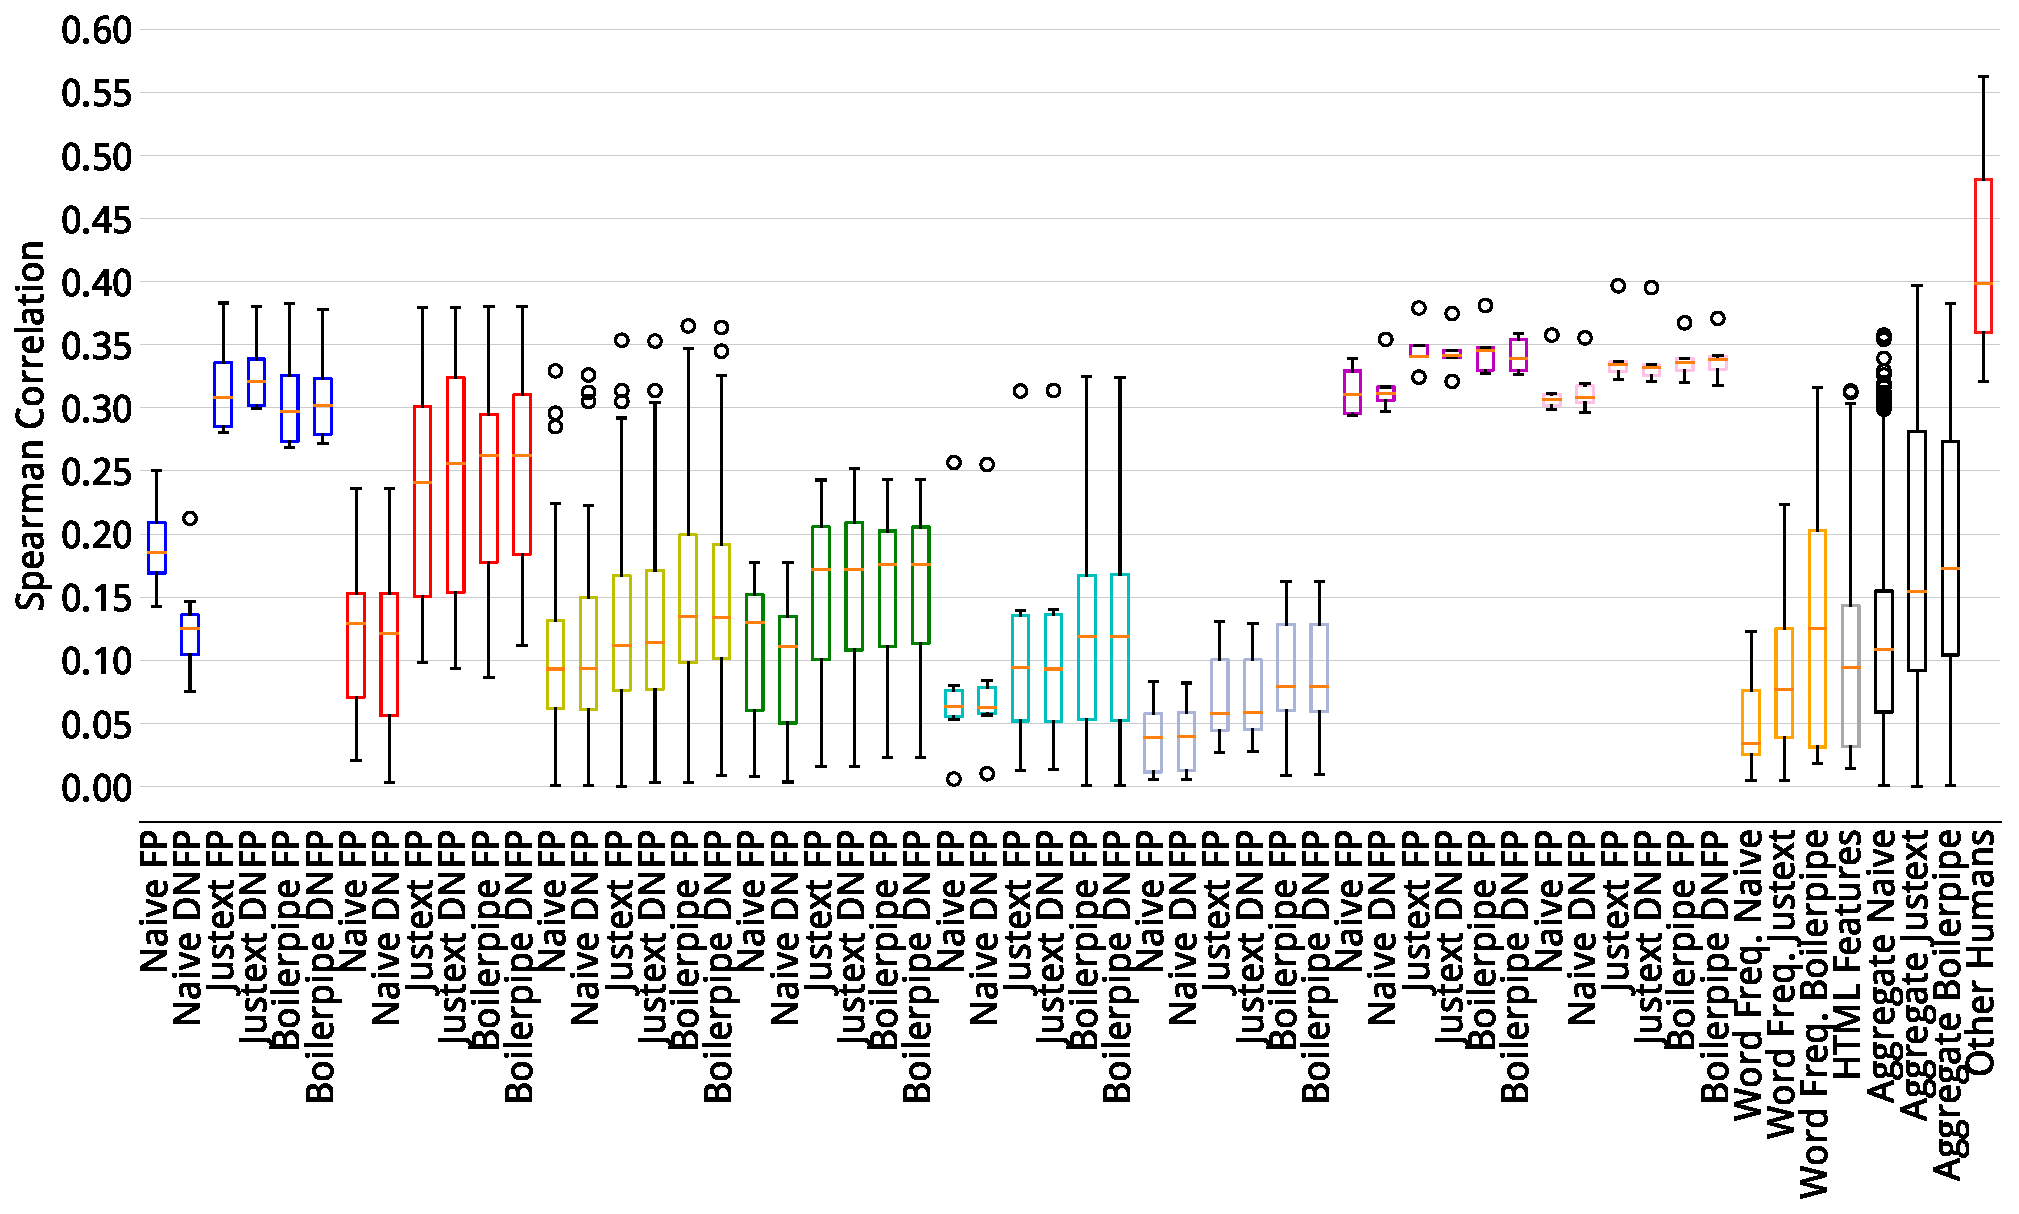
\includegraphics[width=0.90\textwidth]{graphics/box_spearman16_raw_values}
%   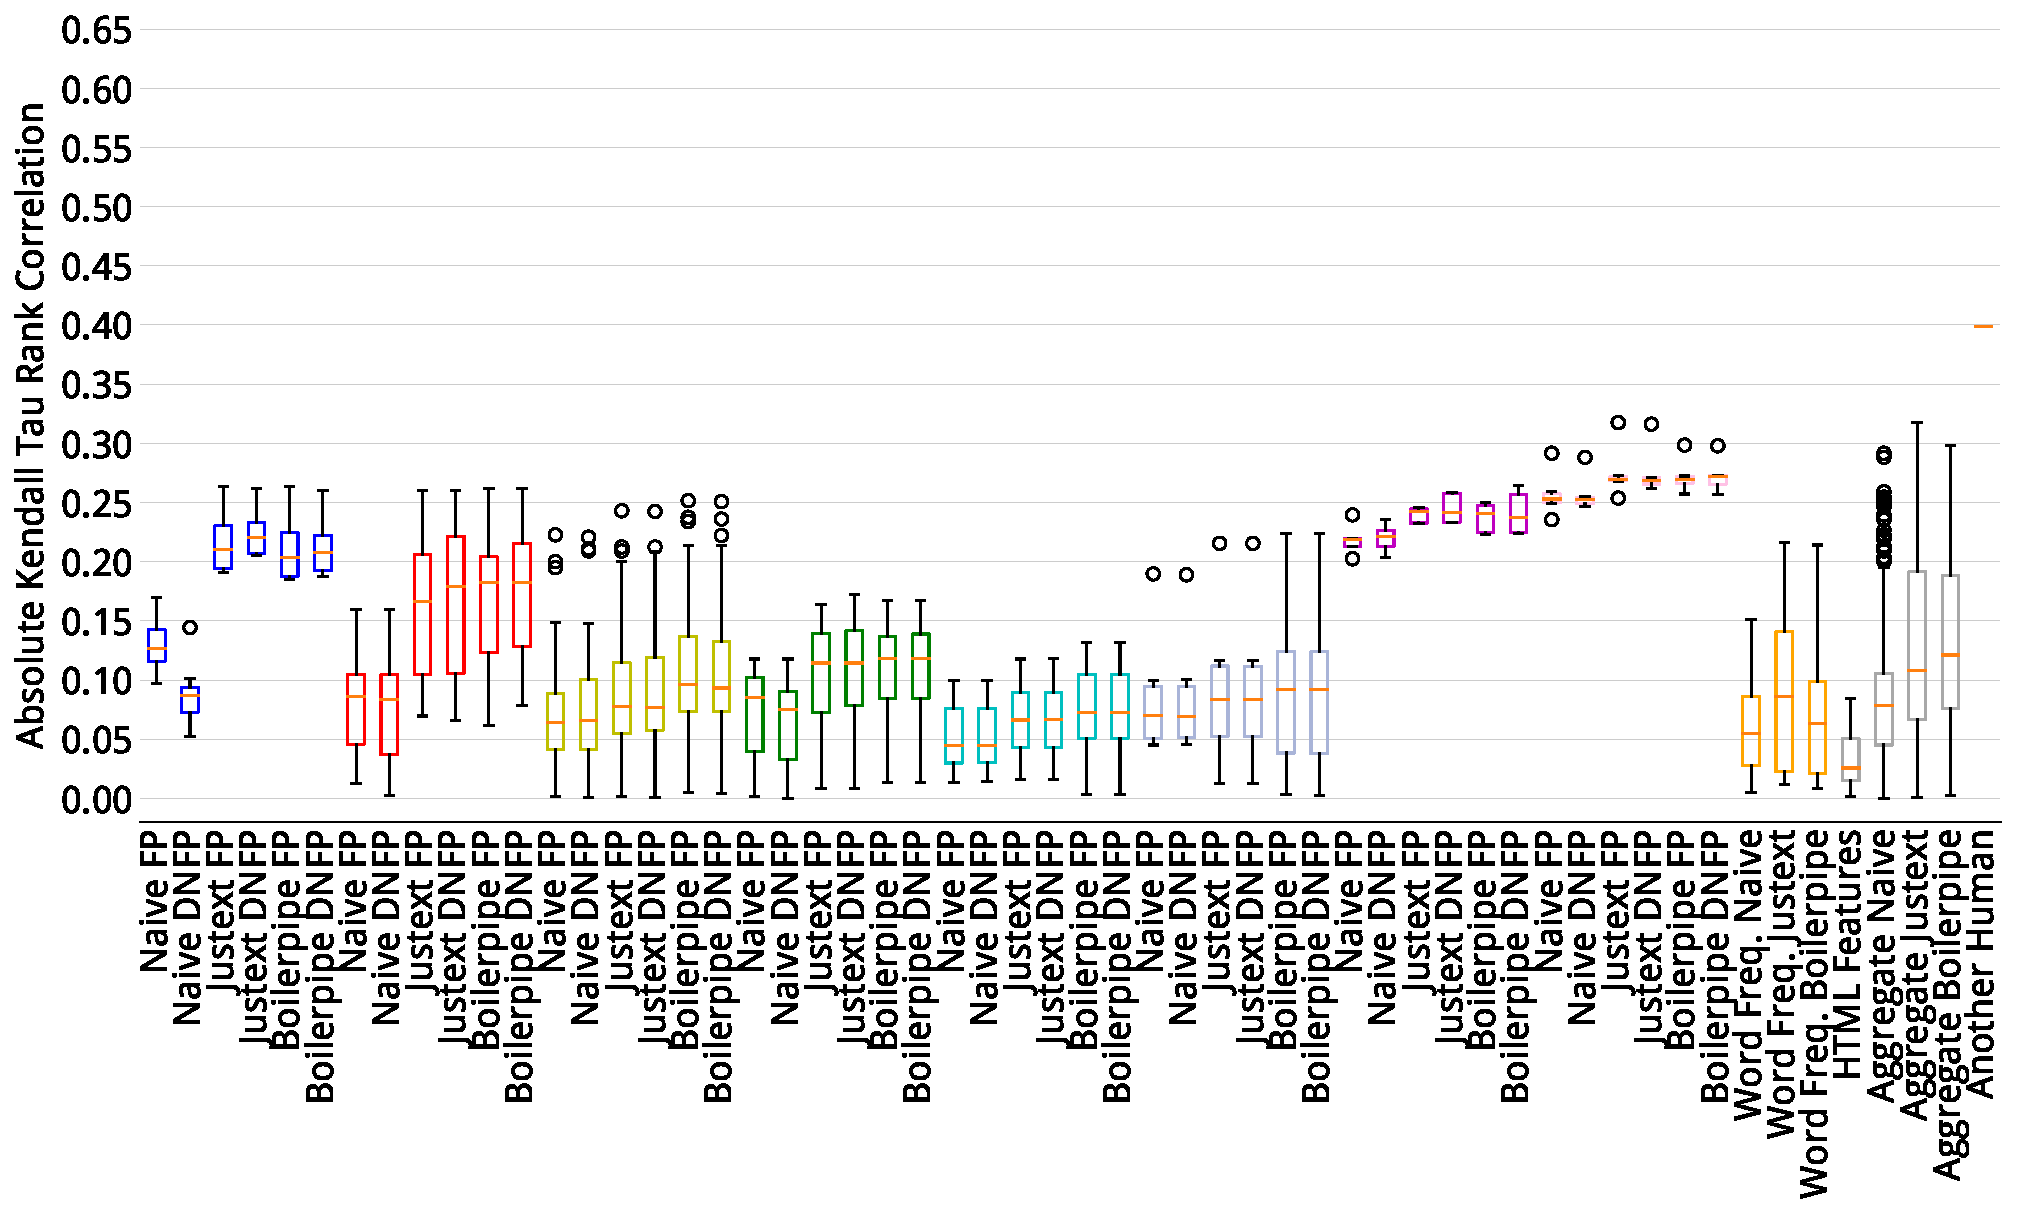
\includegraphics[width=0.90\textwidth]{graphics/box_kendalltau16_raw_values}
%    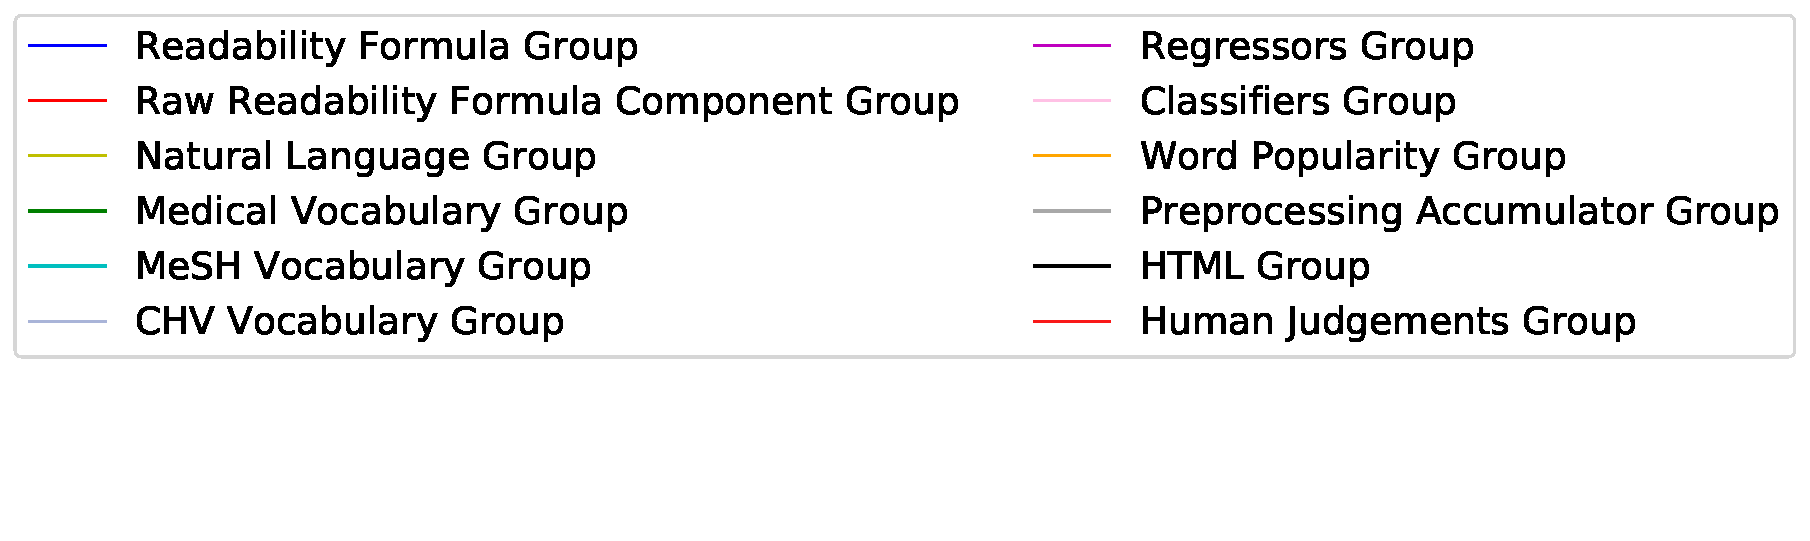
\includegraphics[width=0.65\textwidth]{graphics/legendCorr}
%    \caption{Box plots divided by feature groups. Correlations are calculated using understandability labels from relevant documents assessed in CLEF eHealth 2016}
%   \label{fig:boxplot_corr_docs_2016}
%\end{figure*}

%Figure~\ref{fig:boxplot_corr_docs_2015} shows the correlations for CLEF eHealth 2015 assessments.
Top part of Figure~\ref{fig:boxplot_corr_docs} shows the Spearman correlation for CLEF eHealth 2015 assessments.
The choice of preprocessing method had the highest impact on the traditional readability formula group, with the Naive preprocessing clearly underperforming the other preprocessing methods. The choice of the Naive method was also the worst for the word frequency group, but, interestingly, it was a good choice, or at least a competitive one, for all other groups.
The highest correlations were archived by the regressors and classifiers, independently of the preprocessing method used.

%For this group, all correlation measures point out that the Naive processing yielded the weakest correlation, and Justext was marginally better than Boilerpipe. Comparing the medians, the strategy of DoNotForcePeriod performed better than ForcePeriod. The readability formula group was also the one with higher correlation, with an average correlation equal or higher than the human one.

%Similarly to Figure~\ref{fig:boxplot_corr_docs_2015}, Figure~\ref{fig:boxplot_corr_docs_2016} reports the findings for CLEF eHealth 2016. 
Similarly the bottom part of Figure~\ref{fig:boxplot_corr_docs} reports the findings for CLEF eHealth 2016. 
This time, though, the Naive preprocessing method was clearly underperforming for most of the groups analysed, including regressors and classifiers.

%In order to further understand our experiments, we compared the median of each pair of preprocessing strategy showed in Figures~\ref{fig:boxplot_corr_docs_2015} and~\ref{fig:boxplot_corr_docs_2016} and present the results in Table~\ref{tab:comparison_preprocessing}. 
In order to further understand our experiments, we present in Table~\ref{tab:comparison_preprocessing} the results of comparing the median of two-by-two for different preprocessing strategies shown in Figure~\ref{fig:boxplot_corr_docs}. We also include the results for Pearson and Kendall correlations.
For instance, the entry $\mathit{FP < DNFP}$ counts the number of times the median value for \textit{ForcePeriod} was superior to \textit{DoNotForcePeriod} when comparisons with the same HTML cleaning method was used, e.g. \textit{Naive ForcePeriod} versus \textit{Naive DoNotForcePeriod}. From all comparisons, the ones that were statistically significant according to a t-test are shown inside parentheses.

The upper part of Table~\ref{tab:comparison_preprocessing} shows results for the comparisons between ForcePeriod (FP) and DoNotForcePeriod (DNFP). Although the interpretation of readability formulas is drastically affected by this choice of preprocessing, as research indicates~\cite{palotti15}, the correlation results are not.
The number of times FP reached a higher correlation than DNFP is roughly the same that DNFP was higher than FP.
The bottom part of Table~\ref{tab:comparison_preprocessing} shows the comparisons made for Naive, Justext and Boilerpipe. Results for CLEF 2015 contrast with 2016, while Naive was sightly better than Boilerpipe and Justext in 2015, it was the worst in almost all 2016 comparisons. Also, the comparisons between Justext and Boilerpipe are exactly the opposite from 2015 to 2016.

%
\begin{table}
\centering    
\caption{Exhaustive Comparison summary using the data from Figures 1.2 and 1.3. Numbers inside parentheses represent the number of tests that yielded p < 0.05 in a two-tailed t-test}
\label{tab:comparison_preprocessing}

\resizebox{1.\textwidth}{!}{
\begin{tabular}{lllllllll}
\toprule
\multirow{2}{*}{\textbf{Comparison}} & \multicolumn{4}{c}{\textbf{CLEF 2015}} & \multicolumn{4}{c}{\textbf{CLEF 2016}}\tabularnewline
\cmidrule(l{2pt}r{2pt}){2-5} \cmidrule(l{2pt}r{2pt}){6-9} 
& \textbf{Pearson} & \textbf{Spearman} & \textbf{Kendall Tau} & \textbf{Total} & \textbf{Pearson} & \textbf{Spearman} & \textbf{Kendall Tau} & \textbf{Total}\tabularnewline
\midrule
FP > DNFP & 8 (0) & 11 (4) & 11 (3) & 30 (7) & 16 (10) & 10 (3) & 11 (4) & 37 (17)\tabularnewline
FP < DNFP & 16 (5) & 12 (5) & 12 (6) & 40 (16) & 8 (0) & 12 (2) & 11 (2) & 31 (4)\tabularnewline
FP == DNFP & 0 & 1 & 1 & 2 & 0 & 2 & 2 & 4\tabularnewline
\midrule
Naive > Justext & 11 (7) & 9 (6) & 9 (5) & 29 (18) & 1 (0) & 0 (0) & 0 (0) & 1 (0)\tabularnewline
Naive < Justext & 6 (4) & 8 (4) & 8 (4) & 22 (12) & 16 (12) & 17 (13) & 17 (13) & 50 (38)\tabularnewline
Naive == Justext & 0 & 0 & 0 & 0 & 0 & 0 & 0 & 0\tabularnewline
Naive > Boilerpipe & 12 (7) & 10 (6) & 10 (5) & 32 (18) & 0 (0) & 0 (0) & 0 (0) & 0 (0)\tabularnewline
Naive < Boilerpipe & 5 (4) & 7 (3) & 7 (3) & 19 (10) & 16 (12) & 17 (13) & 17 (13) & 51 (39)\tabularnewline
Naive == Boilerpipe & 0 & 0 & 0 & 0 & 0 & 0 & 0 & 0\tabularnewline
Justext > Boilerpipe & 10 (7) & 16 (9) & 14 (8) & 40 (24) & 9 (4) & 9 (4) & 4 (2) & 17 (8)\tabularnewline
Justext < Boilerpipe & 7 (2) & 1 (0) & 3 (1) & 11 (3) & 8 (2) & 8 (2) & 13 (2) & 34 (6)\tabularnewline
Boilerpipe == Justext & 0 & 0 & 0 & 0 & 0 & 0 & 0 & 0\tabularnewline
\bottomrule 
\end{tabular}
} % close resizebox
\end{table}

%


